\documentclass[sigconf]{acmart}

\acmConference[ACM CAIS]{1st Conference on AI Systems}{June 2026}{San Francisco, CA, USA}
\acmBooktitle{Proceedings of ACM CAIS 2026}
\acmYear{2026}
\acmDOI{}
\acmISBN{}
\settopmatter{printacmref=false}
\setcopyright{none}
\renewcommand\footnotetextcopyrightpermission[1]{}

\usepackage{booktabs}
\usepackage{graphicx}
\usepackage{enumitem}

\graphicspath{{figures/}}

\begin{document}

\title{Arena: Benchmarking AI Agent Frameworks Under Fixed-Model Conditions}
\thanks{Demo video: \url{https://youtu.be/4B-0NkVeUtQ} \\
        Source code: \url{https://github.com/rmilev/arena-acm-cais-2026-demo}}

\author{Roberto Milev}
\affiliation{%
  \institution{Navan}
  \city{Palo Alto}
  \state{CA}
  \country{USA}
}
\email{roberto.milev@navan.com}

\author{Uday Kanagala}
\affiliation{%
  \institution{Navan}
  \city{Palo Alto}
  \state{CA}
  \country{USA}
}
\email{uday.kanagala@navan.com}

\begin{abstract}
Existing agent benchmarks evaluate models, not the frameworks that orchestrate them, making it impossible to isolate how much of an agent's performance comes from the model versus the framework's orchestration code. We present \textbf{Arena}, an open-source benchmarking tool that evaluates agent frameworks under fixed-model conditions. Arena fixes six frameworks---Claude Agent SDK, LangChain, LangGraph, AWS Strands, CrewAI, and Google ADK---to Claude Sonnet~4.5 on AWS Bedrock, connects them to the same MCP tool server, and scores them with a deterministic evaluator across three progressively complex scenarios using six metrics: code complexity, step efficiency, latency, correctness, consistency, and cost. Our evaluation reveals that on simple tasks all frameworks perform comparably, but as complexity increases, traditional frameworks require 2--4$\times$ more orchestration code for multi-agent scenarios yet gain no correctness advantage. The Claude Agent SDK uses a single, unchanged adapter across all three scenarios; only the prompt changes. We contribute (1)~a fixed-model benchmarking methodology that isolates framework behavior from model capability, (2)~an extensible open-source tool for practitioner framework evaluation, and (3)~empirical evidence that model capabilities are beginning to supersede the need for framework orchestration code.
\end{abstract}

\maketitle

%% ============================================================
\section{Introduction}

The AI agent framework landscape is fragmented. Practitioners building tool-using agents must choose between frameworks that differ in abstraction level, orchestration patterns, and developer ergonomics---yet no standard methodology exists for comparing them on equal footing. LangChain~\cite{langchain} and LangGraph provide chain-of-thought orchestration with explicit graph-based control flow. CrewAI~\cite{crewai} offers role-based multi-agent coordination. AWS Strands~\cite{strands} and Google ADK~\cite{adk} provide cloud-native agent runtimes. The Claude Agent SDK~\cite{claudesdk} takes a minimal approach, delegating tool routing, multi-turn orchestration, and even multi-agent coordination entirely to the model.

Existing agent benchmarks---AgentBench~\cite{agentbench}, tau-bench~\cite{taubench}, SWE-bench~\cite{swebench}---evaluate model performance on agent tasks, but they do not control for the framework. When a LangChain agent scores differently from a CrewAI agent, it is unclear whether the difference stems from the model, the framework's orchestration logic, or the interaction between the two. For practitioners making framework adoption decisions, this is the most important question: \emph{holding the model constant, how do frameworks differ?}

We present \textbf{Arena}, an open-source benchmarking tool that fills this gap. Arena evaluates agent frameworks under fixed-model conditions: all six frameworks use Claude Sonnet~4.5 on AWS Bedrock, connect to the same MCP~\cite{mcp} tool server, receive the same system prompt, and are evaluated by the same deterministic scoring rubric. Any measured differences are therefore attributable to the framework's orchestration layer---its tool routing, context management, prompt injection patterns, and multi-agent coordination logic---not the underlying model.

Our evaluation across three progressively complex scenarios reveals a consistent pattern: as task complexity grows, traditional frameworks require progressively more orchestration code---new agent definitions, explicit task decomposition, multi-agent coordination---while the Claude Agent SDK's adapter code remains unchanged. Only the prompt changes. This provides empirical evidence for what we term the \textbf{``prompts not code'' hypothesis}: as model capabilities improve, the value of hand-coded orchestration diminishes.

Our contributions are:
\begin{itemize}[leftmargin=*,nosep]
  \item \textbf{Fixed-model framework benchmarking methodology.} Existing agent benchmarks (AgentBench~\cite{agentbench}, tau-bench~\cite{taubench}, SWE-bench~\cite{swebench}, WebArena~\cite{webarena}, BFCL~\cite{bfcl}) vary the model while holding the task constant. Arena inverts this: by fixing the LLM, tools, prompts, and evaluation criteria, it isolates framework behavior from model capability---a comparison no existing benchmark provides.
  \item \textbf{Arena benchmarking tool.} An open-source, extensible system where practitioners can add their own frameworks, scenarios, and metrics to make informed adoption decisions. Unlike qualitative framework surveys~\cite{masterman} or failure taxonomies~\cite{cemri}, Arena provides controlled quantitative comparison.
  \item \textbf{Empirical evidence for the ``prompts not code'' hypothesis.} Quantitative results across 54~benchmark runs showing that a prompt-driven approach matches or exceeds code-driven orchestration across correctness, consistency, and cost, with 2--4$\times$ less developer code---the first empirical test of whether framework orchestration logic adds value beyond what model capabilities already provide.
\end{itemize}

%% ============================================================
\section{System Architecture}

\subsection{Overview}

Arena is composed of four layers (Figure~\ref{fig:arch}): (1)~a \textbf{tool server layer} implemented as an MCP server providing deterministic tool responses, (2)~a \textbf{framework adapter layer} where each framework implements a common interface to bridge MCP tools into its native format, (3)~a \textbf{benchmark orchestration layer} that executes scenarios with $K$ repetitions and captures metrics including code complexity analysis via Radon~\cite{radon}, and (4)~a \textbf{deterministic evaluator} that scores each run against scenario-specific correctness criteria.

\begin{figure}[t]
  \centering
  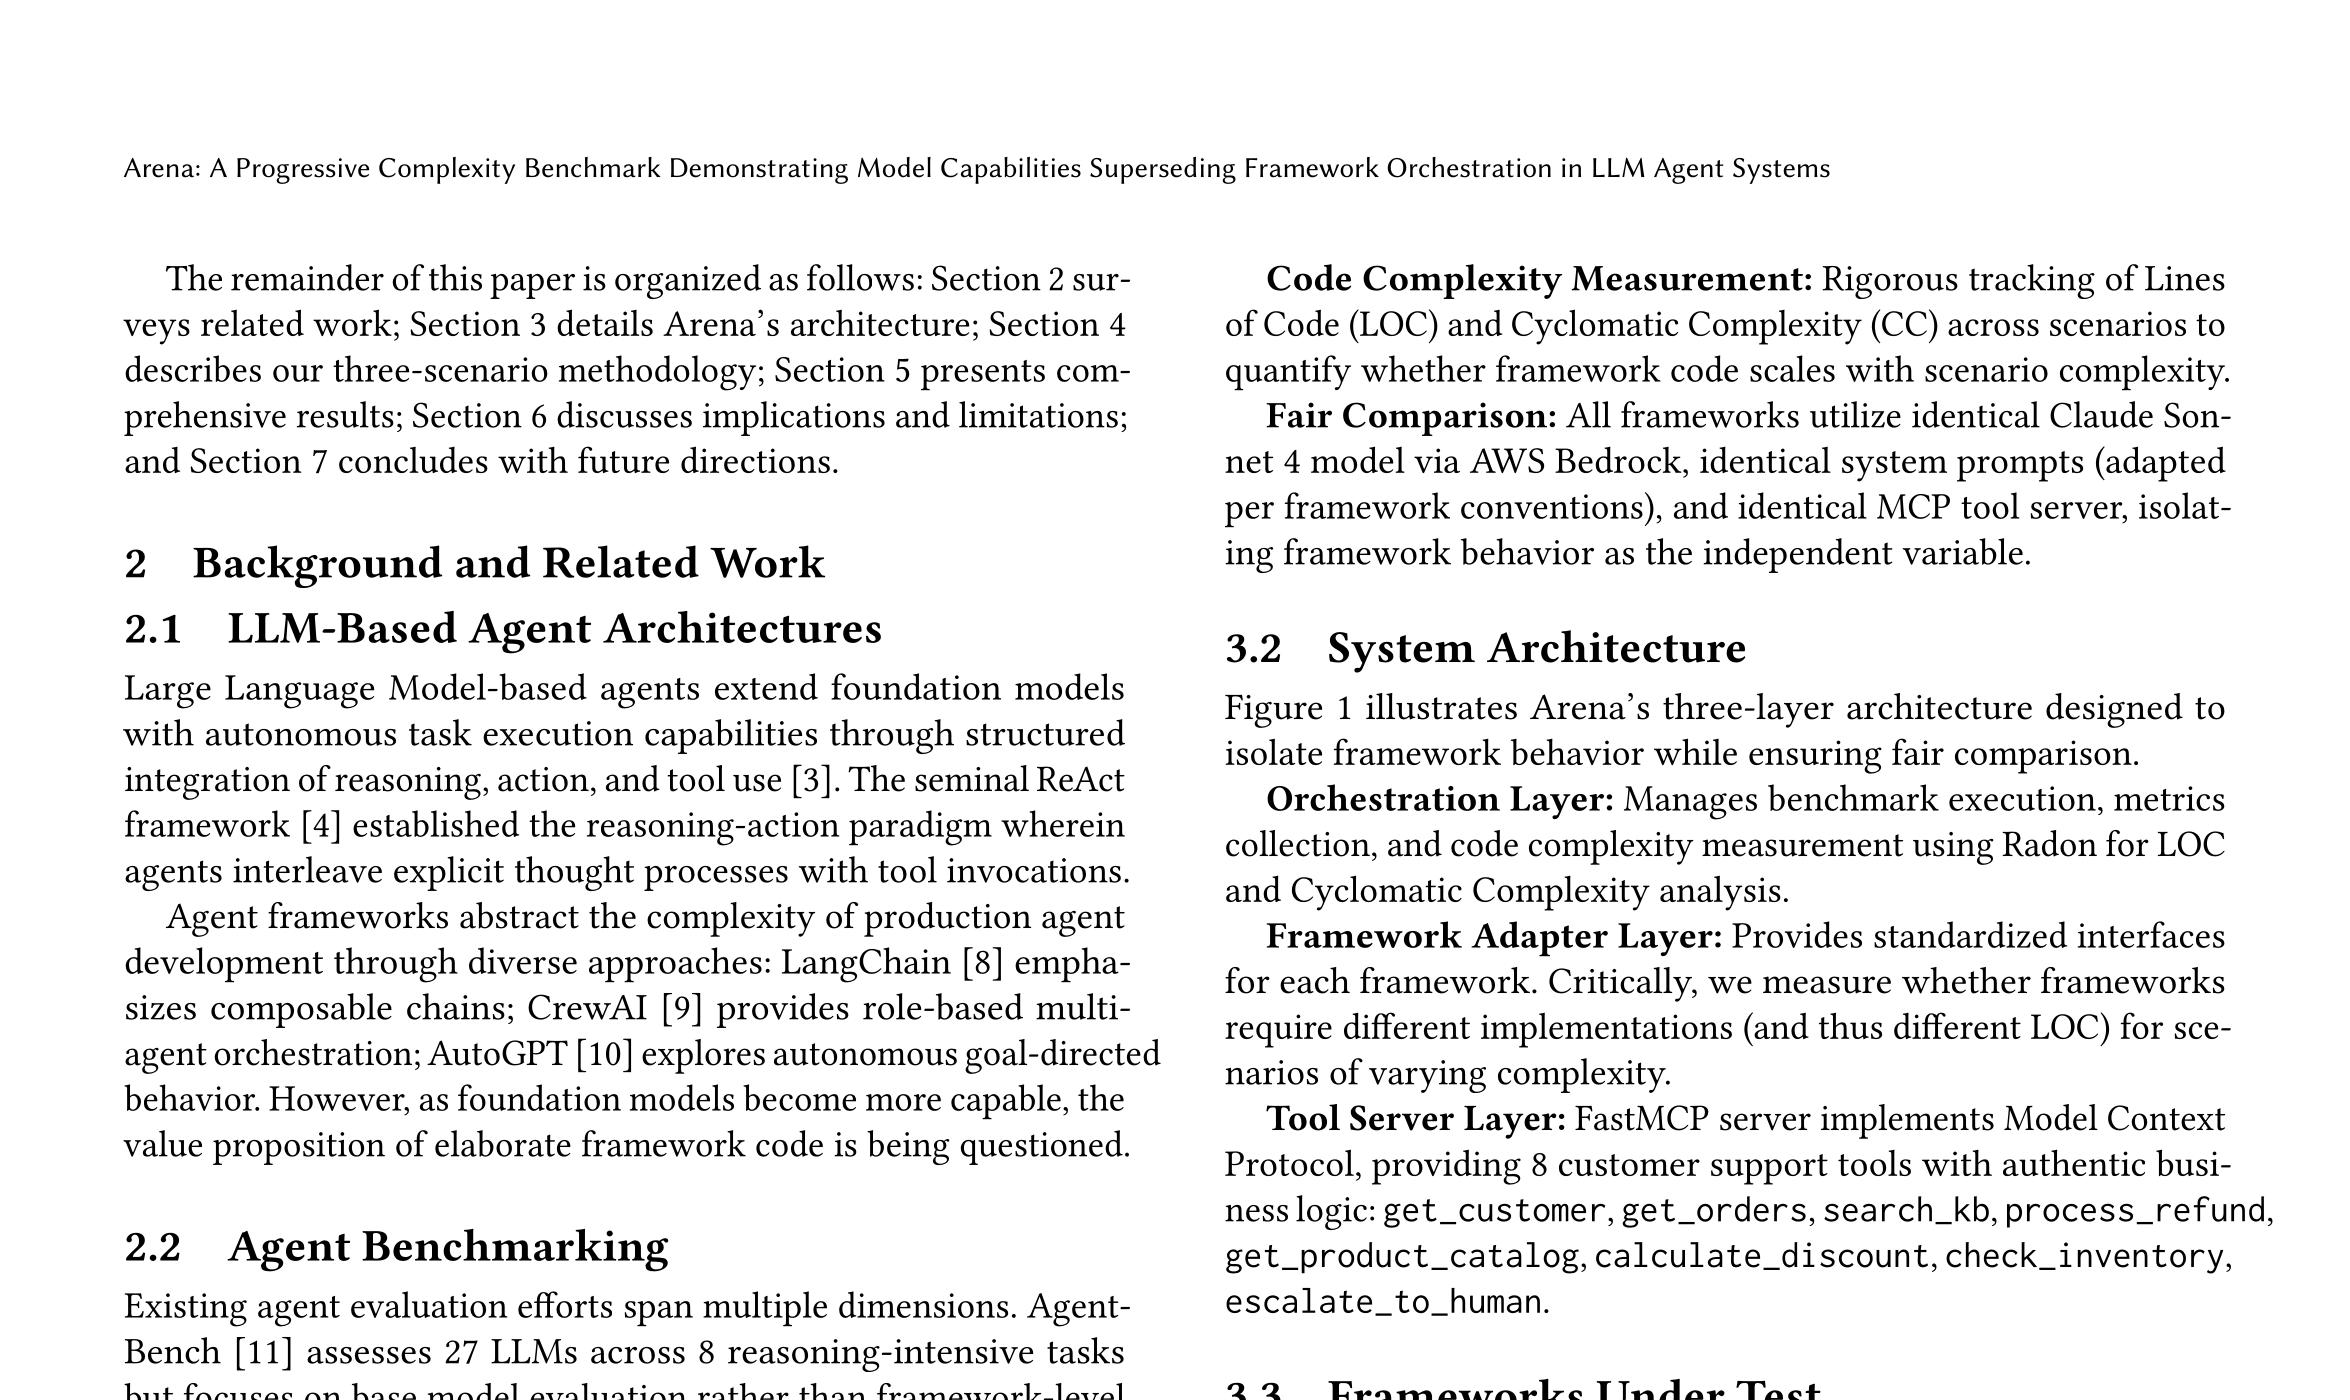
\includegraphics[width=\columnwidth]{fig1_architecture_bw.png}
  \caption{Arena system architecture. All six frameworks connect to the same MCP tool server and are scored by the same deterministic evaluator.}
  \label{fig:arch}
\end{figure}

\subsection{MCP Tool Server}

The backend is a FastMCP~\cite{mcp} server exposing eight domain tools that simulate a customer support system: customer lookup, order retrieval, knowledge base search, refund processing, human escalation, product catalog, discount calculation, and inventory checking. All tools return deterministic JSON responses, ensuring that any variation in agent behavior originates from the framework, not the backend. Two administrative tools (\texttt{arena\_get\_log}, \texttt{arena\_reset\_log}) track the sequence of tool calls made during each run, enabling step efficiency measurement without modifying the framework adapters.

\subsection{Framework Adapters}

Each framework adapter implements a common \texttt{FrameworkAdapter} interface with five methods: MCP server lifecycle (\texttt{start\_mcp\_server}, \texttt{connect\_to\_mcp}), agent execution (\texttt{run\_agent}), and metric collection (\texttt{get\_token\_usage}, \texttt{get\_tool\_log}). This standardized interface ensures that all frameworks are measured identically while allowing each to use its native patterns internally.

The adapter implementations reveal a key structural difference. The Claude Agent SDK adapter passes a system prompt and MCP server configuration to the SDK, which handles the entire tool-use loop internally---approximately 15~lines of substantive code. The other five adapters must manually: (1)~establish and maintain an MCP session, (2)~convert MCP tool schemas into framework-native formats (e.g., Pydantic models for CrewAI, \texttt{StructuredTool} wrappers for LangChain, \texttt{inspect.Signature} bindings for AWS Strands), (3)~configure the LLM client for Bedrock, and (4)~construct the framework's agent/task/crew objects. For multi-agent scenarios, these frameworks additionally require new agent role definitions, task decomposition logic, and coordination code---while the Claude Agent SDK adapter remains unchanged.

\subsection{Metrics}

Arena captures six metrics per run, chosen to cover the concerns practitioners weigh when selecting a framework:

\begin{enumerate}[leftmargin=*,nosep]
  \item \textbf{Code Complexity (LoC + CC):} Lines of code and cyclomatic complexity of each adapter, measured by Radon~\cite{radon}. We measure this \emph{per scenario} to detect whether code scales with task complexity.
  \item \textbf{Step Efficiency:} Ratio of actual tool calls to the optimal sequence defined per scenario. A ratio of 1.0 indicates the agent made exactly the right calls with no redundancy.
  \item \textbf{Latency:} Wall-clock time from prompt submission to final response, including all framework overhead and API round-trips.
  \item \textbf{Correctness:} Rule-based scoring against scenario-specific criteria (e.g., ``did the agent process the refund?''). Scores range from 0.0 to 1.0.
  \item \textbf{Consistency (pass\textsuperscript{3}):} Adapted from tau-bench~\cite{taubench}. Binary: 1.0 only if all $K{=}3$ runs achieve correctness $\geq 0.75$. A single failure drops the score to 0.0, capturing production reliability rather than best-case performance.
  \item \textbf{Cost per Task:} Computed from token usage at standard Anthropic pricing (\$3.00/M~input, \$15.00/M~output).
\end{enumerate}

%% ============================================================
\section{Experimental Setup and Results}

\subsection{Configuration}

All six frameworks use Claude Sonnet~4.5 on AWS Bedrock with temperature$=$0. Each framework receives the same system prompt and connects to the same MCP tool server via stdio transport. We run $K{=}3$ repetitions per scenario per framework, totaling 54~individual runs. Table~\ref{tab:frameworks} shows the frameworks under test.

\begin{table}[t]
  \caption{Frameworks under test.}
  \label{tab:frameworks}
  \small
  \begin{tabular}{ll}
    \toprule
    \textbf{Framework} & \textbf{Adapter Approach} \\
    \midrule
    Claude Agent SDK & Prompt + MCP config; SDK handles orchestration \\
    LangChain & \texttt{ChatBedrockConverse} + \texttt{StructuredTool} \\
    LangGraph & \texttt{create\_react\_agent} graph \\
    AWS Strands & \texttt{BedrockModel} + \texttt{inspect.Signature} \\
    CrewAI & Agent/Task/Crew + Pydantic schemas \\
    Google ADK & \texttt{LlmAgent}/\texttt{Runner} + LiteLLM bridge \\
    \bottomrule
  \end{tabular}
\end{table}

\subsection{Scenarios}

We evaluate three scenarios of increasing complexity. The progressive design is deliberate: S1 establishes that all frameworks are functionally correct, S2 reveals differentiation under realistic complexity, and S3 tests the central hypothesis about code-driven versus prompt-driven orchestration.

\textbf{Scenario~1---Simple Refund (S1).} A customer reports a damaged laptop and requests a refund. Optimal sequence: \texttt{get\_customer} $\rightarrow$ \texttt{get\_orders} $\rightarrow$ \texttt{process\_refund} (3~steps). Purpose: baseline validation.

\textbf{Scenario~2---Multi-Issue Resolution (S2).} A frustrated premium customer presents three simultaneous issues: (1)~a damaged laptop needing a refund, (2)~a double-charged headphone order requiring escalation, and (3)~a shipping address change for an in-transit package. Optimal sequence: 8~tool calls. Purpose: test context management---whether the framework's orchestration layer helps or hinders the model's ability to handle interleaved problems.

\textbf{Scenario~3---Product Investigation (S3).} A customer wants a complete home office upgrade: check refund status, get laptop/monitor/keyboard recommendations, calculate discounts, and stay within a \$3{,}000 budget. Optimal sequence: 12~tool calls. Purpose: the critical test. Traditional frameworks require entirely new multi-agent implementations; the Claude Agent SDK handles it with the same adapter code and a richer prompt.

\subsection{Results}

Table~\ref{tab:results} presents the summary results averaged across all three scenarios.

\begin{table*}[t]
  \caption{Summary results (averaged medians across scenarios, $K{=}3$ runs each).}
  \label{tab:results}
  \small
  \begin{tabular}{lrrrrrrrc}
    \toprule
    \textbf{Framework} & \textbf{LoC} & \textbf{CC} & \textbf{Tokens (In/Out)} & \textbf{Step Eff.} & \textbf{Latency (s)} & \textbf{Correct.} & \textbf{Cost (\$)} & \textbf{pass\textsuperscript{3}} \\
    \midrule
    Claude SDK   & 118 & 3.2 & 18{,}142 / 1{,}828 & 0.67 & 35.06 & 0.87 & 0.084 & 3/3 \\
    LangChain    & 136 & 2.4 & 6{,}517 / 704     & 0.63 & 15.68 & 0.76 & 0.030 & 2/3 \\
    LangGraph    & 136 & 2.4 & 6{,}517 / 760     & 0.63 & 15.92 & 0.76 & 0.031 & 2/3 \\
    AWS Strands  & 141 & 2.4 & 7{,}469 / 758     & 0.67 & 16.85 & 0.84 & 0.034 & 3/3 \\
    CrewAI       & 146 & 1.6 & 6{,}134 / 925     & 0.63 & 18.10 & 0.84 & 0.032 & 3/3 \\
    Google ADK   & 162 & 2.5 & 6{,}803 / 798     & 0.67 & 17.18 & 0.78 & 0.032 & 2/3 \\
    \bottomrule
  \end{tabular}
\end{table*}

\subsubsection{S1: All Frameworks Pass.}
On the simple refund task, all six frameworks achieve 1.0 correctness with optimal step efficiency and pass\textsuperscript{3} consistency across all three runs. Latency ranges from 10.78s (AWS Strands) to 23.32s (Claude SDK), attributable to framework initialization overhead and prompt caching warm-up. This validates the experimental setup and confirms that no framework is fundamentally broken---the real differentiation comes with complexity.

\subsubsection{S2: Frameworks Diverge Under Complexity.}
With the same model, same tools, and same prompt, correctness scores diverge sharply on the multi-issue task. The Claude Agent SDK achieves the highest median correctness (0.88), followed by AWS Strands and CrewAI (0.75 each). LangChain and LangGraph both score 0.50, and Google ADK scores 0.62. Critically, three frameworks---LangChain, LangGraph, and Google ADK---fail the pass\textsuperscript{3} consistency check on S2, meaning at least one of their three runs scored below 0.75. The framework's orchestration layer---specifically how it manages context across interleaved problems---measurably affects outcomes.

\subsubsection{S3: The Code Complexity Inflection.}
Scenario~3 produces the paper's central finding (Figure~\ref{fig:loc_correctness}). The Claude Agent SDK adapter is identical to S1 and S2---118~lines of code, unchanged. Only the prompt changes. All other frameworks require entirely new multi-agent implementations with explicit agent role definitions, task decomposition, coordination logic, and result aggregation. All six frameworks converge to 0.77 correctness on S3, demonstrating that the additional orchestration code provides no correctness advantage.

\begin{table}[t]
  \caption{Adapter code growth across scenarios.}
  \label{tab:growth}
  \small
  \begin{tabular}{lrrl}
    \toprule
    \textbf{Framework} & \textbf{S1/S2} & \textbf{S3} & \textbf{Growth} \\
    \midrule
    Claude SDK   & 118 & 118 & 1.0$\times$ \\
    LangChain    & 136 & 190 & 1.4$\times$ \\
    LangGraph    & 136 & 225 & 1.7$\times$ \\
    AWS Strands  & 141 & 267 & 1.9$\times$ \\
    CrewAI       & 146 & 228 & 1.6$\times$ \\
    Google ADK   & 162 & 236 & 1.5$\times$ \\
    \bottomrule
  \end{tabular}
\end{table}

\noindent Despite requiring 1.4--1.9$\times$ more orchestration code (190--267~LoC in entirely new files), the traditional frameworks achieve identical correctness to the Claude Agent SDK on S3 (0.77 across all six). The Claude Agent SDK, using the same 118-line adapter with a richer prompt, matches the explicit multi-agent implementations. This demonstrates that the model's native planning and tool-routing capabilities can substitute for hand-coded orchestration logic.

\begin{figure}[t]
  \centering
  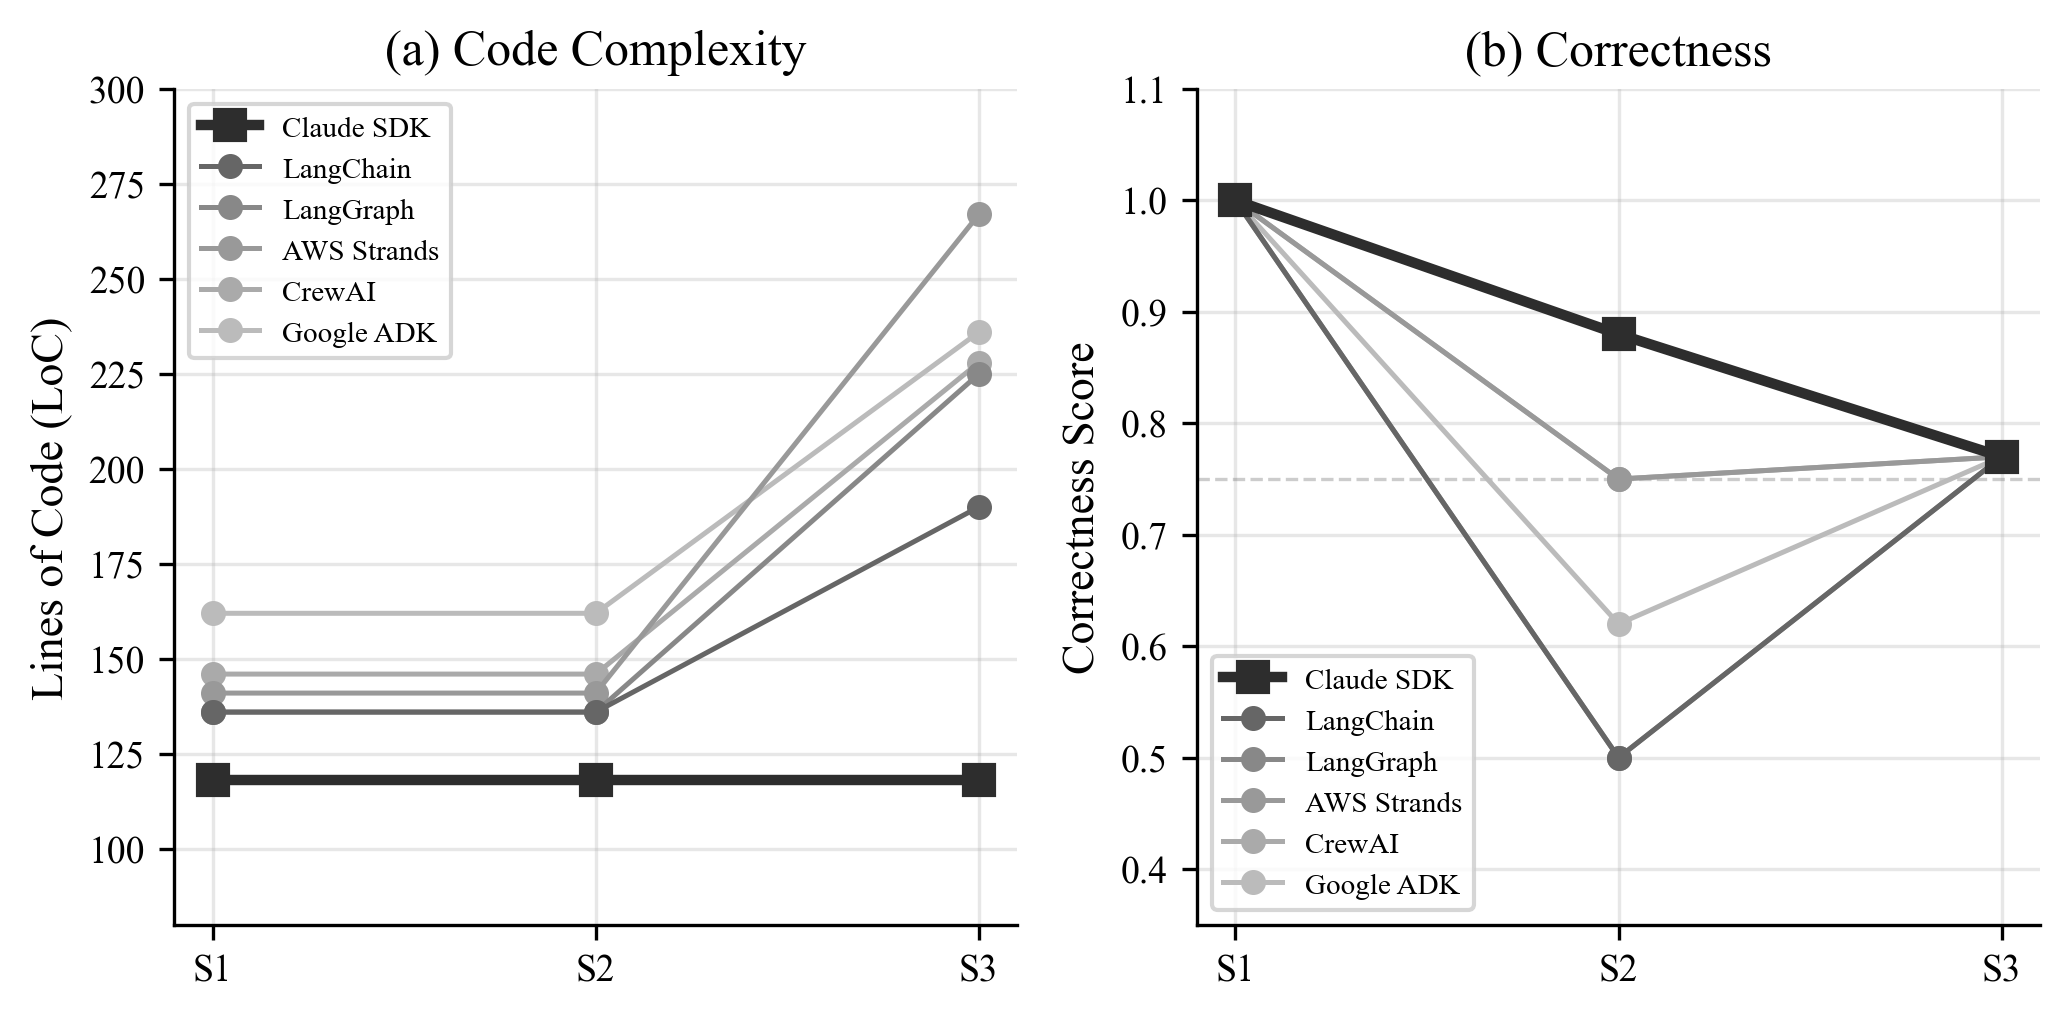
\includegraphics[width=\columnwidth]{fig4_loc_vs_correctness.png}
  \caption{Code complexity vs.\ correctness across S1/S2/S3. The Claude Agent SDK (flat line) achieves the highest average correctness with constant code complexity.}
  \label{fig:loc_correctness}
\end{figure}

%% ============================================================
\section{Discussion}

\subsection{The ``Prompts Not Code'' Paradigm}

Our results suggest a paradigm shift in agent development. The traditional approach (2023--2024) requires explicit framework orchestration: agent roles defined in code, parallel coordination through programming constructs, code complexity scaling with scenario complexity. The emerging approach delegates these responsibilities to the model through natural language: agent roles defined in prompts, parallel coordination through model reasoning, code complexity remaining constant.

The evidence (Figure~\ref{fig:loc_correctness}): Claude Agent SDK maintains 118~lines of adapter code across all three scenarios while achieving the highest average correctness (0.87). The five traditional frameworks require 190--267~lines of new code for S3 yet all converge to identical correctness (0.77). The Claude Agent SDK achieves this through 2.7$\times$ higher token consumption (18{,}142 vs.\ 6{,}500--7{,}500 input tokens per task), trading compute cost for developer effort---a trade-off that becomes increasingly favorable as API costs decline and developer costs rise.

\subsection{When Frameworks Still Matter}

Prompt-driven orchestration is not a universal replacement. Frameworks remain valuable for constraints the model cannot enforce: rate limiting, authentication, compliance logging, deterministic routing guarantees, and integration with existing CI/CD and observability infrastructure. For production systems with strict operational requirements, the framework's runtime---not its orchestration logic---is the differentiator.

\subsection{Practitioner Guidance}

Based on our results, we offer the following guidance:
\begin{itemize}[leftmargin=*,nosep]
  \item \textbf{For prototyping and evolving requirements:} Prefer prompt-driven approaches (Claude Agent SDK). The constant code footprint means new scenarios require prompt changes, not new implementations.
  \item \textbf{For latency-sensitive applications:} The five traditional frameworks cluster at 15--18s average latency versus 35s for Claude SDK. AWS Strands and LangChain are fastest.
  \item \textbf{For explicit orchestration visibility:} Frameworks like CrewAI and LangGraph provide transparent agent role definitions and task graphs that are easier to audit and debug.
\end{itemize}

\subsection{Limitations}

Our evaluation uses a single model (Claude Sonnet~4.5), a single domain (customer support), and a simulated backend (not real APIs). The ``prompts not code'' finding may be specific to highly capable models---less capable models may still benefit from framework-level orchestration. Arena is designed to be extensible: practitioners can add models, domains, and scenarios to test generalizability. Framework versions evolve rapidly; our implementations reflect March~2026 releases.

%% ============================================================
\section{Demonstration Scenario}

We demonstrate Arena with two interaction modes designed to showcase both the tool's capabilities and the ``prompts not code'' finding.

\textbf{Mode~A: Live Benchmark Run.}
An attendee selects a scenario complexity level (S1, S2, or S3) and a subset of frameworks. Arena executes the benchmark in real-time, displaying per-run metrics as they complete: tool call sequences, token counts, latency, correctness scores, and cost. The results table populates live, allowing direct comparison across frameworks on identical tasks.

\textbf{Mode~B: Side-by-Side Code Comparison.}
We display the Claude Agent SDK adapter alongside a traditional framework adapter (e.g., CrewAI) for the same scenario. For~S1, the audience sees that the Claude SDK adapter is a prompt and an MCP server configuration ($\sim$15~lines of substantive code), while the CrewAI adapter involves MCP connection management, Pydantic model generation, async/sync bridging, and agent/task/crew construction ($\sim$146~lines). For~S3, we show how the traditional adapter requires an entirely new multi-agent implementation while the Claude SDK adapter remains unchanged---only the prompt evolves.

\textbf{Audience Interaction.} Attendees can suggest modifications to the scenario (e.g., adding a new customer issue) and observe how each framework's adapter must change to accommodate it---or in the Claude SDK's case, how only the prompt changes.

\begin{figure}[t]
  \centering
  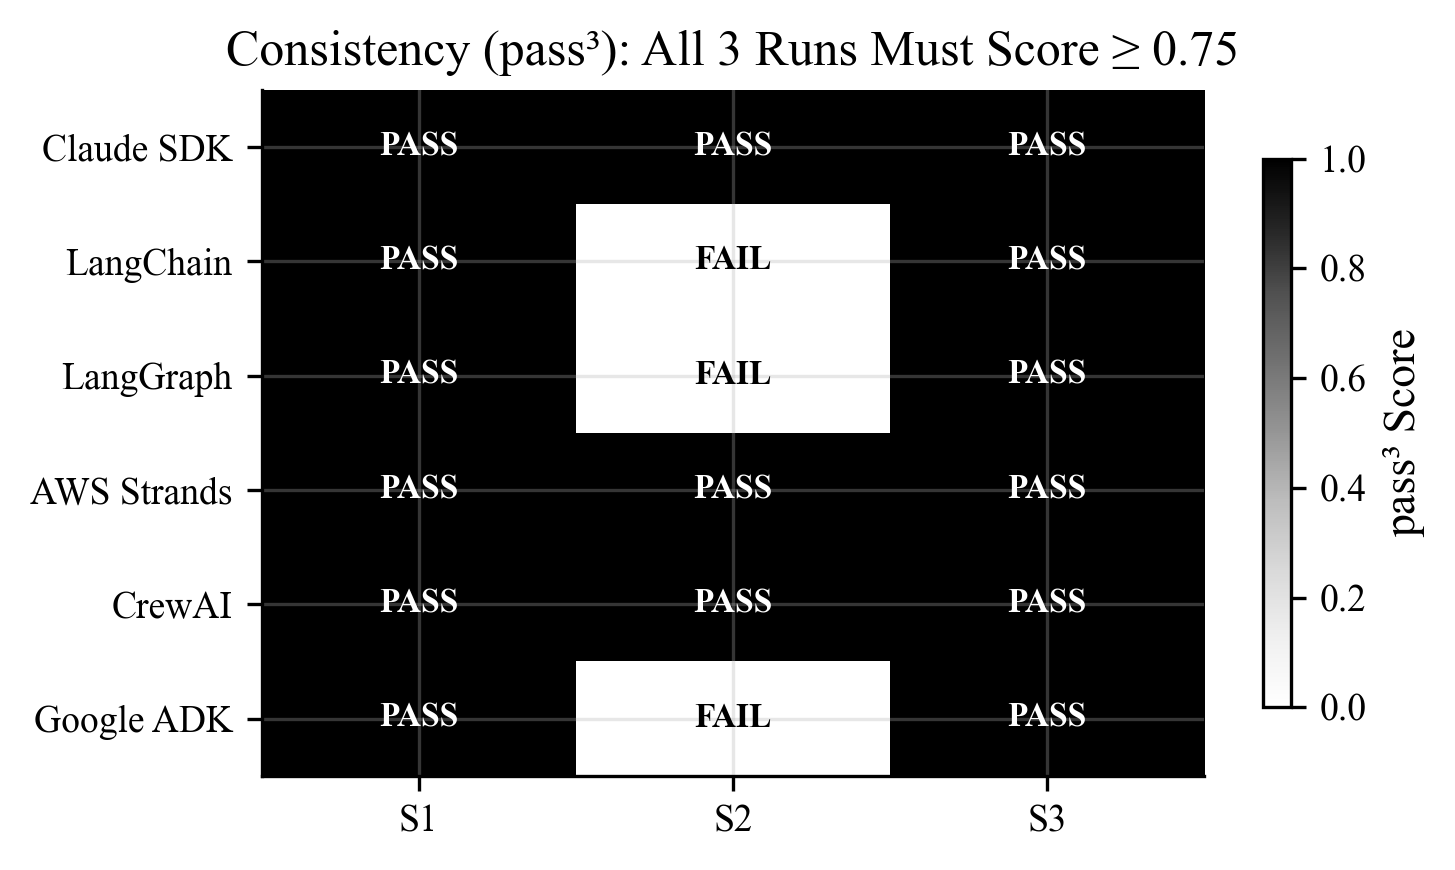
\includegraphics[width=\columnwidth]{fig6_consistency.png}
  \caption{Pass\textsuperscript{3} consistency heatmap. Green indicates all three runs passed ($\geq$0.75 correctness). LangChain, LangGraph, and Google ADK fail on S2.}
  \label{fig:consistency}
\end{figure}

%% ============================================================
\section{Related Work}

\textbf{Agent benchmarks.} AgentBench~\cite{agentbench} evaluates LLMs across 8 interactive environments but focuses on model comparison rather than framework comparison. tau-bench~\cite{taubench} introduces the pass\textsuperscript{$k$} reliability metric for retail and airline domains, which we adopt as pass\textsuperscript{3}. SWE-bench~\cite{swebench} benchmarks autonomous code repair. WebArena~\cite{webarena} provides realistic web environments for agent evaluation. The Berkeley Function Calling Leaderboard~\cite{bfcl} evaluates tool-use accuracy across models. All of these benchmarks vary the model while holding the task constant; Arena inverts this by holding the model constant and varying the framework. To our knowledge, no existing benchmark isolates framework behavior under fixed-model conditions.

\textbf{Framework evaluation and multi-agent failure analysis.} Cemri et~al.~\cite{cemri} analyze 1{,}600+ execution traces across seven multi-agent frameworks, identifying 14~failure modes in three categories: system design issues, inter-agent misalignment, and task verification failures. Their finding that framework design choices are a primary driver of agent failures directly motivates Arena's controlled comparison methodology. Masterman et~al.~\cite{masterman} survey emerging agent architectures, cataloging single-agent and multi-agent design patterns---the same patterns Arena benchmarks empirically. AutoGen~\cite{autogen} introduced conversable multi-agent patterns now adopted by several frameworks under test. However, none of these works benchmarks frameworks against each other with a fixed model.

\textbf{Agent cost and evaluation methodology.} Kapoor et~al.~\cite{kapoor} demonstrate that agents vary by 100$\times$ in cost for equivalent tasks and advocate for accuracy-cost Pareto analysis. We adopt their multi-metric philosophy, including cost as a first-class metric. Yao et~al.~\cite{react} established the ReAct reasoning-action pattern that underlies most frameworks under test; Verma et~al.~\cite{verma} later showed that ReAct's gains stem from exemplar-query similarity rather than genuine interleaved reasoning, supporting our hypothesis that model capability matters more than orchestration pattern.

\textbf{Tool protocols.} The Model Context Protocol (MCP)~\cite{mcp} provides a standardized interface between agents and tools. Arena uses MCP as the common tool layer, ensuring all frameworks access identical capabilities and eliminating tool integration as a confounding variable.

%% ============================================================
\bibliographystyle{ACM-Reference-Format}
\begin{thebibliography}{18}

\bibitem{langchain}
LangChain.
\newblock LangChain: Build context-aware reasoning applications.
\newblock \url{https://www.langchain.com/}, 2024.

\bibitem{crewai}
J.~P.~S. Moura.
\newblock CrewAI: Framework for orchestrating role-playing autonomous AI agents.
\newblock \url{https://www.crewai.com/}, 2024.

\bibitem{strands}
AWS.
\newblock AWS Strands Agents SDK.
\newblock \url{https://github.com/strands-agents/sdk-python}, 2025.

\bibitem{adk}
Google.
\newblock Google Agent Development Kit (ADK).
\newblock \url{https://google.github.io/adk-docs/}, 2025.

\bibitem{claudesdk}
Anthropic.
\newblock Claude Agent SDK.
\newblock \url{https://github.com/anthropics/claude-agent-sdk-python}, 2025.

\bibitem{agentbench}
X.~Liu et~al.
\newblock AgentBench: Evaluating LLMs as agents.
\newblock In \emph{ICLR}, 2024.

\bibitem{taubench}
S.~Yao, N.~Shinn, P.~Razavi, and K.~Narasimhan.
\newblock tau-bench: A benchmark for tool-agent-user interaction in real-world domains.
\newblock \emph{arXiv preprint arXiv:2406.12045}, 2024.

\bibitem{swebench}
C.~E. Jimenez et~al.
\newblock SWE-bench: Can language models resolve real-world GitHub issues?
\newblock In \emph{ICLR}, 2024.

\bibitem{mcp}
Anthropic.
\newblock Model Context Protocol specification.
\newblock \url{https://modelcontextprotocol.io/}, 2024.

\bibitem{cemri}
M.~Cemri, M.~Z.~Pan, S.~Yang, et~al.
\newblock Why do multi-agent LLM systems fail?
\newblock \emph{arXiv preprint arXiv:2503.13657}, 2025.

\bibitem{masterman}
T.~Masterman, S.~Besen, M.~Sawtell, and A.~Chao.
\newblock The landscape of emerging AI agent architectures for reasoning, planning, and tool calling: A survey.
\newblock \emph{arXiv preprint arXiv:2404.11584}, 2024.

\bibitem{kapoor}
S.~Kapoor, B.~Stroebl, Z.~S.~Siegel, N.~Nadgir, and A.~Narayanan.
\newblock AI agents that matter.
\newblock \emph{arXiv preprint arXiv:2407.01502}, 2024.

\bibitem{radon}
M.~Lacchia.
\newblock Radon: Python tool for computing code metrics.
\newblock \url{https://radon.readthedocs.io/}, 2023.

\bibitem{webarena}
S.~Zhou et~al.
\newblock WebArena: A realistic web environment for building autonomous agents.
\newblock In \emph{ICLR}, 2024.

\bibitem{bfcl}
F.~Yan et~al.
\newblock Berkeley Function Calling Leaderboard.
\newblock \emph{arXiv preprint arXiv:2402.14848}, 2024.

\bibitem{autogen}
Q.~Wu et~al.
\newblock AutoGen: Enabling next-gen LLM applications via multi-agent conversation.
\newblock In \emph{COLM}, 2024.

\bibitem{react}
S.~Yao et~al.
\newblock ReAct: Synergizing reasoning and acting in language models.
\newblock In \emph{ICLR}, 2023.

\bibitem{verma}
M.~Verma, S.~Bhambri, and S.~Kambhampati.
\newblock On the brittle foundations of ReAct prompting for agentic large language models.
\newblock \emph{arXiv preprint arXiv:2405.13966}, 2024.

\end{thebibliography}

\end{document}
